\section{The DREAM framework}
\label{sec:method}

% --- Fig 2 system diagram (TikZ) ----------------------------------------
% Fig 2 — DREAM system diagram (TikZ skeleton).
%
% Manual draw element — refine line widths, fonts, and labels in final paper.
% Designed as full-width (0.95\textwidth) horizontal flow with 6 boxes + arrows.
%
% Compile in the main paper with:  % Fig 2 — DREAM system diagram (TikZ skeleton).
%
% Manual draw element — refine line widths, fonts, and labels in final paper.
% Designed as full-width (0.95\textwidth) horizontal flow with 6 boxes + arrows.
%
% Compile in the main paper with:  % Fig 2 — DREAM system diagram (TikZ skeleton).
%
% Manual draw element — refine line widths, fonts, and labels in final paper.
% Designed as full-width (0.95\textwidth) horizontal flow with 6 boxes + arrows.
%
% Compile in the main paper with:  \input{figures/paper/fig2_system_diagram.tex}
%
\begin{figure*}[t]
\centering
\begin{tikzpicture}[
    node distance=14mm and 8mm,
    box/.style={
        rectangle, rounded corners, draw, fill=gray!8,
        minimum width=23mm, minimum height=14mm,
        font=\small, align=center,
    },
    src/.style={box, fill=blue!8, draw=blue!50!black},
    out/.style={box, fill=green!8, draw=green!50!black},
    arr/.style={-{Latex[length=2mm]}, semithick},
]
% Row of 6 lanes
\node[src]                  (data)  {Data lane\\\footnotesize FAA · USGS · OSM\\\footnotesize adsb.lol · METAR};
\node[box, right=of data]   (geom)  {Geometry\\\footnotesize OLS $\to$ 3-D SDF\\\footnotesize Vertiport OFV};
\node[box, right=of geom]   (traf)  {Traffic\\\footnotesize Runway-config\\\footnotesize Dynamic envelope};
\node[box, right=of traf]   (ml)    {ML\\\footnotesize Counterfactual\\\footnotesize XGB + conformal};
\node[box, right=of ml]     (plan)  {Planning\\\footnotesize Envelope-aware A*\\\footnotesize 5-term cost};
\node[out, right=of plan]   (eval)  {Analysis\\\footnotesize Safety / Capacity\\\footnotesize / Accessibility KPI};

% Top-row inputs to geometry + traffic + ml
\draw[arr] (data) -- (geom);
\draw[arr] (data.east) to[bend right=12] (traf.west);
\draw[arr] (data.east) to[bend right=22] (ml.west);

\draw[arr] (geom) -- (traf);
\draw[arr] (geom.east) to[bend right=12] (ml.west);
\draw[arr] (geom.east) to[bend right=22] (plan.west);

\draw[arr] (traf) -- (ml);
\draw[arr] (traf.east) to[bend right=12] (plan.west);

\draw[arr] (ml)   -- (plan);
\draw[arr] (plan) -- (eval);

% Footer label
\node[font=\footnotesize, below=4mm of plan.south] (capnote)
    {DREAM pipeline. All lanes ship a \texttt{sanity\_check} entry-point exercised by \texttt{scripts/run\_sanity.py}.};
\end{tikzpicture}
\caption{DREAM framework lanes. Real airport / ADS-B / weather data flow through
    six lanes culminating in safety/capacity/accessibility KPIs. The geometry
    lane encodes ICAO Annex~14 as a 3-D signed-distance field; the traffic lane
    converts ADS-B into a runway-configuration-aware dynamic envelope; the ML
    lane learns a risk field by counterfactual injection; planning runs an
    envelope-constrained A* over a 5-term cost.}
\label{fig:dream-pipeline}
\end{figure*}

%
\begin{figure*}[t]
\centering
\begin{tikzpicture}[
    node distance=14mm and 8mm,
    box/.style={
        rectangle, rounded corners, draw, fill=gray!8,
        minimum width=23mm, minimum height=14mm,
        font=\small, align=center,
    },
    src/.style={box, fill=blue!8, draw=blue!50!black},
    out/.style={box, fill=green!8, draw=green!50!black},
    arr/.style={-{Latex[length=2mm]}, semithick},
]
% Row of 6 lanes
\node[src]                  (data)  {Data lane\\\footnotesize FAA · USGS · OSM\\\footnotesize adsb.lol · METAR};
\node[box, right=of data]   (geom)  {Geometry\\\footnotesize OLS $\to$ 3-D SDF\\\footnotesize Vertiport OFV};
\node[box, right=of geom]   (traf)  {Traffic\\\footnotesize Runway-config\\\footnotesize Dynamic envelope};
\node[box, right=of traf]   (ml)    {ML\\\footnotesize Counterfactual\\\footnotesize XGB + conformal};
\node[box, right=of ml]     (plan)  {Planning\\\footnotesize Envelope-aware A*\\\footnotesize 5-term cost};
\node[out, right=of plan]   (eval)  {Analysis\\\footnotesize Safety / Capacity\\\footnotesize / Accessibility KPI};

% Top-row inputs to geometry + traffic + ml
\draw[arr] (data) -- (geom);
\draw[arr] (data.east) to[bend right=12] (traf.west);
\draw[arr] (data.east) to[bend right=22] (ml.west);

\draw[arr] (geom) -- (traf);
\draw[arr] (geom.east) to[bend right=12] (ml.west);
\draw[arr] (geom.east) to[bend right=22] (plan.west);

\draw[arr] (traf) -- (ml);
\draw[arr] (traf.east) to[bend right=12] (plan.west);

\draw[arr] (ml)   -- (plan);
\draw[arr] (plan) -- (eval);

% Footer label
\node[font=\footnotesize, below=4mm of plan.south] (capnote)
    {DREAM pipeline. All lanes ship a \texttt{sanity\_check} entry-point exercised by \texttt{scripts/run\_sanity.py}.};
\end{tikzpicture}
\caption{DREAM framework lanes. Real airport / ADS-B / weather data flow through
    six lanes culminating in safety/capacity/accessibility KPIs. The geometry
    lane encodes ICAO Annex~14 as a 3-D signed-distance field; the traffic lane
    converts ADS-B into a runway-configuration-aware dynamic envelope; the ML
    lane learns a risk field by counterfactual injection; planning runs an
    envelope-constrained A* over a 5-term cost.}
\label{fig:dream-pipeline}
\end{figure*}

%
\begin{figure*}[t]
\centering
\begin{tikzpicture}[
    node distance=14mm and 8mm,
    box/.style={
        rectangle, rounded corners, draw, fill=gray!8,
        minimum width=23mm, minimum height=14mm,
        font=\small, align=center,
    },
    src/.style={box, fill=blue!8, draw=blue!50!black},
    out/.style={box, fill=green!8, draw=green!50!black},
    arr/.style={-{Latex[length=2mm]}, semithick},
]
% Row of 6 lanes
\node[src]                  (data)  {Data lane\\\footnotesize FAA · USGS · OSM\\\footnotesize adsb.lol · METAR};
\node[box, right=of data]   (geom)  {Geometry\\\footnotesize OLS $\to$ 3-D SDF\\\footnotesize Vertiport OFV};
\node[box, right=of geom]   (traf)  {Traffic\\\footnotesize Runway-config\\\footnotesize Dynamic envelope};
\node[box, right=of traf]   (ml)    {ML\\\footnotesize Counterfactual\\\footnotesize XGB + conformal};
\node[box, right=of ml]     (plan)  {Planning\\\footnotesize Envelope-aware A*\\\footnotesize 5-term cost};
\node[out, right=of plan]   (eval)  {Analysis\\\footnotesize Safety / Capacity\\\footnotesize / Accessibility KPI};

% Top-row inputs to geometry + traffic + ml
\draw[arr] (data) -- (geom);
\draw[arr] (data.east) to[bend right=12] (traf.west);
\draw[arr] (data.east) to[bend right=22] (ml.west);

\draw[arr] (geom) -- (traf);
\draw[arr] (geom.east) to[bend right=12] (ml.west);
\draw[arr] (geom.east) to[bend right=22] (plan.west);

\draw[arr] (traf) -- (ml);
\draw[arr] (traf.east) to[bend right=12] (plan.west);

\draw[arr] (ml)   -- (plan);
\draw[arr] (plan) -- (eval);

% Footer label
\node[font=\footnotesize, below=4mm of plan.south] (capnote)
    {DREAM pipeline. All lanes ship a \texttt{sanity\_check} entry-point exercised by \texttt{scripts/run\_sanity.py}.};
\end{tikzpicture}
\caption{DREAM framework lanes. Real airport / ADS-B / weather data flow through
    six lanes culminating in safety/capacity/accessibility KPIs. The geometry
    lane encodes ICAO Annex~14 as a 3-D signed-distance field; the traffic lane
    converts ADS-B into a runway-configuration-aware dynamic envelope; the ML
    lane learns a risk field by counterfactual injection; planning runs an
    envelope-constrained A* over a 5-term cost.}
\label{fig:dream-pipeline}
\end{figure*}


DREAM is a five-stage pipeline running on each airport's local
east-north-up (ENU) frame centred at the aerodrome reference point (ARP).
All spatial quantities are in metres unless otherwise stated; altitudes are
above mean sea level unless explicitly annotated as above ground level. The
five stages are: (i) static Annex~14 obstacle protection as a signed-distance
field; (ii) runway-configuration inference from real ADS-B; (iii) the dynamic
safety envelope $\Edyn$; (iv) counterfactual-injection risk-field learning;
and (v) envelope-constrained corridor planning. \Cref{fig:dream-pipeline}
shows the lane decomposition.

\subsection{Annex 14 OLS as a signed-distance field}
\label{sec:method-sdf}

Let $\mathcal{R}_a$ denote the set of runway ends at airport $a$, with
threshold-to-end vectors $\mathbf{r}^{thr}_{i}, \mathbf{r}^{end}_{i}$
in ENU for runway end $i \in \mathcal{R}_a$. For each runway end and each of
the nine Annex~14 surface families (approach, takeoff climb, transitional,
inner horizontal, conical, runway strip, runway-end safety area, OFZ inner
approach, OFZ inner transitional), we construct a 3-D prism whose footprint
is a trapezoid (approach/takeoff/transitional/OFZ), an annulus
(inner horizontal/conical), or a rectangle (runway strip/RESA), and whose
upper face is given by the family's affine slope. \Cref{tab:ols-params}
records the parameter values; they are the publicly documented Code~4
precision-approach values, not a copy of the ICAO normative text. A
per-airport YAML override under \texttt{configs/annex14/} supports
airport-specific calibration.

We sample the union of all prisms onto a regular voxel grid centred on the
ARP and store the resulting signed-distance values as a 32-bit array:

\begin{equation}
\dOLS(\mathbf{p}) \;=\; \min_{i}\; \mathrm{sdist}\bigl(\mathbf{p}, P_i\bigr),
\quad
\mathbf{p}=(x,y,z) \in \R^3,
\label{eq:sdf}
\end{equation}

where $P_i$ ranges over all prisms and $\mathrm{sdist}$ returns the
signed distance to a single prism (negative inside, positive outside). For
LAX and SFO, $\dOLS$ lives on a $600 \times 600 \times 117$ voxel grid
covering a $60\,\mathrm{km} \times 60\,\mathrm{km}$ ARP-centred box from
$0$ to $3\,500$~m at $100$~m horizontal and $30$~m vertical resolution.
Building $\dOLS$ for an entire airport takes $\sim\!45$~s of single-thread
Python. The \texttt{is\_clear} and \texttt{clearance\_m} queries used by
downstream stages are constant-time trilinear lookups.

\Cref{fig:ols-3d} renders the $98$ prisms making up the LAX SDF on its 8
runways (4 parallel pairs, 06/24 and 07/25), together with each
runway-strip centroid.

% --- Fig 3 OLS 3D rendering --------------------------------------------
\begin{figure}[t]
    \centering
    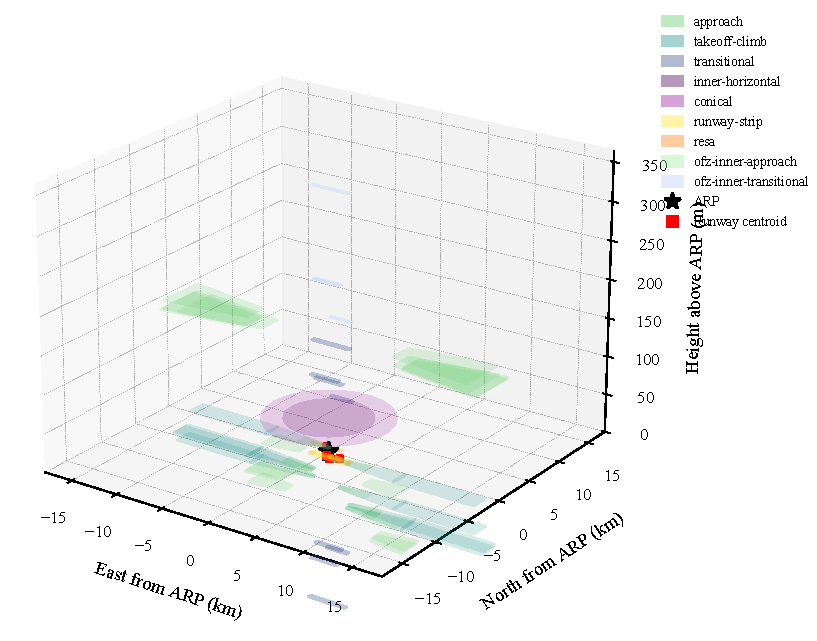
\includegraphics[width=\linewidth]{../figures/paper/fig3_ols_3d_klax.pdf}
    \caption{Annex 14 OLS for LAX (\texttt{KLAX}) rendered as the
        top-of-prism polygons of the 98 prisms underlying the signed-distance
        field of \cref{eq:sdf}. Approach, takeoff-climb, transitional,
        inner-horizontal, conical, runway-strip, RESA, and OFZ surfaces are
        coloured per family; the ARP is marked $\star$ and the runway
        centroids in red.}
    \label{fig:ols-3d}
\end{figure}

% --- Table 4 OLS parameters --------------------------------------------
\begin{table}[t]
\centering
\caption{Annex 14 OLS parameters used by DREAM (generic Code 4 precision approach). These are public-secondary-source placeholder values, not a copy of the ICAO normative text. Per-airport calibration is supported via the YAML override in \texttt{configs/annex14/}.}
\label{tab:ols-params}
\begin{tabular}{lr}
\toprule
Parameter & Value \\
\midrule
Approach surface (inner edge / divergence) & 300 m / 0.150 rad \\
Approach section 1 (slope $\times$ length) & 1:50 $\times$ 3000 m \\
Approach section 2 (slope $\times$ length) & 1:40 $\times$ 3600 m \\
Takeoff-climb (slope $\times$ length) & 1:50 $\times$ 15000 m \\
Transitional slope & 1:7 \\
Inner horizontal (radius / height) & 4000 m / 45 m \\
Conical (slope / height) & 1:20 / 100 m \\
Runway strip (half-width / end length) & 150 m / 60 m \\
Runway end safety area (RESA) & 240 $\times$ 150 m \\
OFZ inner-approach (slope $\times$ length) & 1:50 $\times$ 900 m \\
OFZ inner-transitional slope & 1:3 \\
Vertiport approach/departure (slope, FAA EB-105A) & 1:8 \\
Vertiport OFV (FATO half-side / height) & 16 m / 300 m \\
\bottomrule
\end{tabular}
\end{table}


\paragraph{Vertiport obstacle-free volumes (OFV).}
Each candidate vertiport $v \in \{V_1, V_2, V_3, V_4\}$ has a local FATO and
a funnel-shaped OFV with $8{:}1$ slope above it~\citep{faa_eb_105a}. We build
a per-vertiport SDF on a tight $400 \times 400 \times 400$~m box at
$10$~m resolution and snap each corridor endpoint to a voxel that is both
clear of all Annex~14 surfaces and inside the OFV
funnel~\citep{easa_vertiport_proto}.

\subsection{ADS-B-driven runway-configuration inference}
\label{sec:method-config}

We process raw ADS-B state vectors $\bigl(\text{lat}, \text{lon},
\text{baro\_alt}, \text{velocity}, \text{vertical\_rate}, \text{track},
\text{on\_ground}\bigr)$ from the \texttt{adsb.lol} historical archive
(\cref{sec:data}). After WGS-84$\rightarrow$ENU projection, outlier rejection
(speed jumps $>200$~m/s, altitude jumps $>1000$~m/step, duplicate timestamps),
and a 5-s resample per ICAO24, we classify each track as one of
\{\textsc{arrival}, \textsc{departure}, \textsc{overflight}\} by a rule on
vertical rate, distance to the ARP, and a sliding-window minimum of
$d_{\mathrm{runway}}(\mathbf{p})$. Each classified track is assigned to the
closest runway end whose extension line contains the track's entry (for
arrivals) or exit (for departures) point within a $\pm15^\circ$ bearing
tolerance.

A 15-minute rolling vote then yields the active arrivals and departures at
time $t$:

\begin{equation}
\Rt \;=\; \bigl( \text{arr}_t, \text{dep}_t \bigr),
\quad
\text{arr}_t = \argmax_{r \in \mathcal{R}_a}\!\sum_{\tau \in [t-\Delta, t]} \1[\textsc{arrival}_\tau \mapsto r],
\label{eq:Rt}
\end{equation}

with $\Delta = 15$~min and an analogous expression for $\text{dep}_t$. A
slice is called \emph{confident} if the winning runway end exceeds a
$70\,\%$ share of operations in that slice or the top-2 vote is consistent
for three consecutive slices.

\paragraph{METAR cross-check.}
We validate $\Rt$ against the contemporaneous METAR wind by requiring the
predicted active landing direction to lie within $\pm 60^\circ$ of the
METAR-reported mean wind. On real LAX + SFO operational data
(\cref{sec:data,sec:lax,sec:sfo}) this cross-check matches on
$28/29 = 96.6\,\%$ of scoreable slices across our ten airport-days.

\subsection{The dynamic safety envelope $\Edyn$}
\label{sec:method-envelope}

We define the static both-sides-closed Annex 14 mask
\begin{equation}
\Astatic
\;=\;
\bigl\{
\mathbf{p} : \dOLS(\mathbf{p}) > \Delta_{\mathrm{safe}}
\bigr\}
\;\cap\;
\bigl\{
\mathbf{p} \notin \mathcal{S}_{\mathrm{rwy}}
\bigr\},
\label{eq:Astatic}
\end{equation}
where $\mathcal{S}_{\mathrm{rwy}}$ is the union of $3\,\NM \times 1\,500\,\ft$
protective corridors centred on every runway centreline at every parallel-runway
airport, regardless of which runway is currently active. The closure
$\mathcal{S}_{\mathrm{rwy}}$ is the price the planner pays for being
\emph{runway-configuration-blind} -- a planner that has only Annex~14
geometry to work with must protect both sides because it cannot tell which
side is in use.

The \emph{dynamic} closure is then the time-varying subset of
$\mathcal{S}_{\mathrm{rwy}}$ that is actually justified by the current
runway configuration:
\begin{equation}
\Cdyn
\;=\;
g(\Rt, \Wt, \Ft)
\;\subseteq\;
\mathcal{S}_{\mathrm{rwy}},
\label{eq:Cdyn}
\end{equation}
where $\Wt$ is the contemporaneous METAR and $\Ft$ is the
voxelised arrival/departure density (\cref{sec:method-config}). Under
instrument-meteorological conditions ($\text{visibility} < 5$~km or
$\text{ceiling} < 1000$~ft), $\Cdyn$ is laterally expanded by $25\,\%$ to
absorb the ADS-B and ATC uncertainty inherent in IMC operations.

The DREAM safety envelope is the difference
\begin{equation}
\boxed{\Edyn \;=\; \Astatic \setminus \Cdyn},
\label{eq:Edyn}
\end{equation}
the space the planner may use \emph{operationally} at time $t$.

\Cref{fig:envelope-filmstrip} renders $\Edyn$ at four representative UTC
hours of a single Friday at LAX at $\sim1\,500$~ft AGL. The closed regions
rotate with the active configuration. We note explicitly that
$\Edyn \subseteq \Astatic$, so every $\Edyn$-feasible corridor is also
$\Astatic$-feasible if the planner is given the additional information of
$\Rt$. The empirical question, which we answer in \cref{sec:lax,sec:sfo},
is how often \emph{the converse} ($\Astatic$-feasible but $\Edyn$-infeasible)
versus \emph{the additional} ($\Edyn$-feasible but $\Astatic$-infeasible)
direction matters in practice. We will see that the additional direction --
configuration awareness reopening pairs that the both-sides-closed baseline
forbids -- dominates.

% --- Fig 4 envelope filmstrip -------------------------------------------
\begin{figure*}[t]
    \centering
    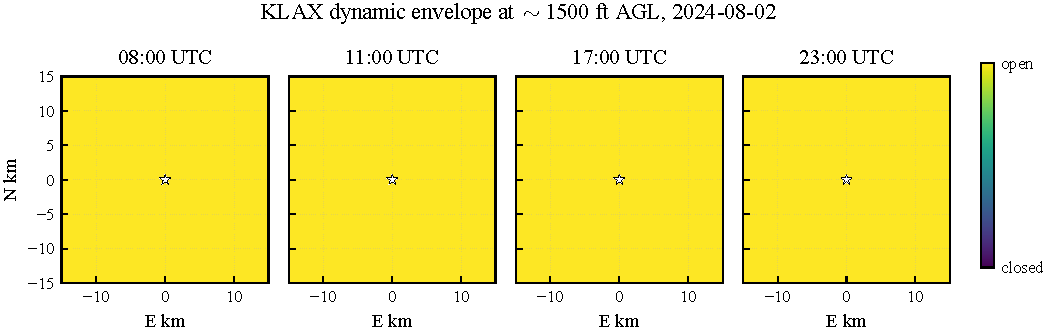
\includegraphics[width=\linewidth]{../figures/paper/fig4_envelope_filmstrip_klax.pdf}
    \caption{LAX dynamic envelope $\Edyn$ at $\sim1\,500$~ft AGL on
        2024-08-02 at four UTC hours. Yellow~=~open for eVTOL traffic;
        purple~=~closed by the runway-configuration-aware envelope. The
        closure pattern rotates with the active runway configuration
        $\Rt$ inferred from real ADS-B.}
    \label{fig:envelope-filmstrip}
\end{figure*}

\subsection{Counterfactual-injection risk field}
\label{sec:method-risk}

Within a single 15-min slice we sample candidate eVTOL trajectories
$\sigma_{j,t}$ inside $\Astatic \cap \Edyn$ from a uniform random origin in
$\Vofv^{(v_1)}$ to a uniform random destination elsewhere in $\Astatic$,
linearly interpolated with a constant climb/descent profile from
\texttt{configs/scenarios/cost\_weights.yaml}. Each segment is labelled
$y_{j,t} = 1$ if any of the five \emph{deterministic} conflict criteria fires
against contemporaneous real fixed-wing ADS-B:
\begin{enumerate}
    \item lateral separation $< 1.5\,\NM$ \emph{and} vertical separation
    $< 1\,000\,\ft$ to any active ADS-B track within $\pm 60$~s;
    \item the segment crosses the active runway axis below $2\,000$~ft AGL;
    \item the segment intersects the active approach prism;
    \item the segment intersects the active departure prism;
    \item the SDF margin $\dOLS$ at the midpoint drops below
    $\Delta_{\mathrm{safe}}$.
\end{enumerate}
Otherwise $y_{j,t} = 0$. The labels are \emph{deterministic}: they are
defined by the OLS geometry and the actual contemporaneous ADS-B positions,
not by a surrogate model.

We extract a 12-dimensional feature vector per segment midpoint
\(\mathbf{x}_{j,t}=(\dOLS, d_{rwy}, d_{app}, d_{dep},
\rho_{\mathrm{traffic}},
\sin(\theta_w), \cos(\theta_w),
v_w, \mathrm{vis}, \mathrm{ceil}, \sin(2\pi h/24), \cos(2\pi h/24))\),
extended with a one-hot encoding of the active runway-configuration tag, and
train logistic regression (LR), random forest (RF), gradient boosting (XGB),
and a 4-layer multilayer perceptron (MLP) on the resulting tabular dataset.

\paragraph{Temporal hold-out.}
We hold out the last Friday of the window (2024-08-30) as a temporal test
day and train on the preceding four Fridays. To convert the classifier
probabilities into calibrated prediction sets, we use split-conformal
prediction with target coverage $1-\alpha = 0.90$
\citep{vovk_conformal,angelopoulos2021gentle}.

\subsection{Envelope-constrained planning}
\label{sec:method-planner}

The 3-D ENU voxel graph $G_t = (N_t, E_t)$ has one node per voxel cell
$(x_i, y_j, z_k)$ inside $\Edyn$, and 26-connected edges subject to
climb-rate and turn-rate caps from \texttt{cost\_weights.yaml}. The planner
solves the constrained shortest-path problem
\begin{equation}
\pi^\star
=
\argmin_{\pi \subset G_t}
\sum_{e_{ij}\in\pi}
\Bigl[
\alpha_1 T_{ij} + \alpha_2 E_{ij} + \alpha_3 \rhof_{ij} + \alpha_4 N_{ij} + \alpha_5 I_{ij}
\Bigr],
\label{eq:objective}
\end{equation}
where $T_{ij}$ is the segment flight time, $E_{ij}$ a quadratic energy proxy,
$\rhof_{ij}$ the conformal-calibrated risk-field probability,
$N_{ij}$ a noise-exposure proxy (population-weighted), and $I_{ij}$ a
runway-throughput-impact proxy. We solve \cref{eq:objective} with a vanilla
$A^\star$ whose heuristic is the ENU $\ell_2$ distance divided by cruise
speed.

\paragraph{Baselines.}
We define five baselines that gate which terms of \cref{eq:objective} are
active and which mask is the feasibility constraint:
\begin{description}
\item[$B_0$:] no-eVTOL operations. Records the conventional fixed-wing
    operations on the day but plans no eVTOL corridor.
\item[$B_1$:] straight-line corridor between vertiport pairs, ignoring
    every spatial constraint. Always feasible by construction. Captures the
    naive ``low-altitude routing'' framing.
\item[$B_2$:] $A^\star$ over $\Astatic$ only. The
    \emph{runway-configuration-blind, Annex-14-only} baseline. This is the
    operational state of an UAM planner that has been given Annex~14 geometry
    but no live runway-configuration data; it must close both parallel-runway
    corridors as a pessimistic safety measure.
\item[$B_3$:] $A^\star$ over $\Edyn = \Astatic \setminus \Cdyn$. The
    \emph{runway-configuration-aware} dynamic envelope. Uses the inferred
    $\Rt$ and the METAR $\Wt$ to reopen the off-side corridor of every
    parallel-runway pair.
\item[$B_4$:] $B_3$ plus the risk-field term $\rhof_{ij}$ as an additional
    soft cost. Documented here for completeness; the per-corridor risk-grid
    export is left as immediate future work
    (\cref{sec:discussion}).
\end{description}

The headline experimental question of this paper -- and the one to which we
return in \cref{sec:lax,sec:sfo} -- is the gap between $B_2$ and $B_3$.

\subsection{Counterfactual injection as honest framing}
\label{sec:method-counterfactual}

We close the methods section with a remark on framing. No large-scale
commercial eVTOL service exists at LAX or SFO today; we therefore cannot
\emph{compare} simulated and real eVTOL behaviour. We can, however, ask the
\emph{counterfactual} question: \textit{had a candidate eVTOL segment flown
through the airport at this time slice, would it have conflicted with the
fixed-wing traffic that did fly?} The answer is determined by the actual
ADS-B trajectories and the deterministic conflict criteria of
\cref{sec:method-risk}; it does not require a learned surrogate for eVTOL
behaviour. We adopt this framing throughout and avoid the phrase ``real
eVTOL data'' in our experimental claims.
